\chapter{Progettazione del Software}

La \textbf{Progettazione del Software} è il processo di definizione dell'architettura, dei componenti, delle interfacce e di altri attributi di un sistema o di un componente. È una fase cruciale nel ciclo di vita dello sviluppo del software, che traduce i requisiti in un piano dettagliato per la costruzione del sistema.

\section{Analisi dei Requisiti}
L'\textbf{analisi dei requisiti} è il processo di definizione, documentazione e mantenimento dei requisiti software. È la fase iniziale di qualsiasi progetto software e mira a comprendere le esigenze degli stakeholder per il sistema da costruire.

\subsection{Tipi di Requisiti}
I requisiti possono essere classificati in due categorie principali:
\begin{itemize}
    \item \textbf{Requisiti Funzionali}: Descrivono ciò che il sistema \textit{deve fare}. Definiscono le funzioni, i servizi e i comportamenti specifici che il sistema deve fornire agli utenti.
    \begin{itemize}
        \item \textbf{Esempi}: "Il sistema deve consentire la registrazione di nuovi utenti.", "Il sistema deve calcolare la somma delle vendite giornaliere.", "Il sistema deve permettere la visualizzazione del calendario delle partite."
    \end{itemize}
    \item \textbf{Requisiti Non Funzionali (o di Qualità)}: Descrivono come il sistema \textit{deve funzionare}. Definiscono le caratteristiche di qualità, i vincoli e gli attributi del sistema, piuttosto che le sue funzionalità specifiche. Spesso influenzano l'architettura e l'implementazione.
    \begin{itemize}
        \item \textbf{Esempi}:
        \begin{itemize}
            \item \textbf{Prestazioni}: "Il sistema deve rispondere a una query entro 2 secondi."
            \item \textbf{Scalabilità}: "Il sistema deve supportare 1000 utenti concorrenti."
            \item \textbf{Sicurezza}: "Il sistema deve autenticare gli utenti tramite username e password con criptazione."
            \item \textbf{Usabilità}: "L'interfaccia utente deve essere intuitiva e di facile apprendimento."
            \item \textbf{Affidabilità}: "Il sistema deve essere disponibile il 99.9\% del tempo."
            \item \textbf{Manutenibilità}: "Il codice deve essere modulare e ben documentato."
            \item \textbf{Portabilità}: "Il sistema deve funzionare su Windows e Linux."
        \end{itemize}
    \end{itemize}
\end{itemize}

\subsection{Diagrammi di Casi d'Uso UML (Use Case Diagrams)}
I \textbf{Diagrammi di Casi d'Uso} sono uno strumento UML (Unified Modeling Language) utilizzato nell'analisi dei requisiti funzionali. Descrivono le interazioni tra gli utenti (attori) e il sistema, rappresentando le diverse funzionalità che il sistema offre dal punto di vista dell'utente.
\begin{itemize}
    \item \textbf{Componenti Principali}:
    \begin{itemize}
        \item \textbf{Attore (Actor)}: Rappresenta un ruolo esterno che interagisce con il sistema (persona, altro sistema, dispositivo). Disegnato come un omino stilizzato.
        \item \textbf{Caso d'Uso (Use Case)}: Rappresenta una funzionalità specifica del sistema, un servizio che il sistema fornisce all'attore. Disegnato come un ovale.
        \item \textbf{Confine del Sistema (System Boundary)}: Un rettangolo che racchiude i casi d'uso, distinguendo ciò che è all'interno del sistema da ciò che è esterno.
        \item \textbf{Relazioni}:
        \begin{itemize}
            \item \textbf{Associazione}: L'interazione tra un attore e un caso d'uso (linea semplice).
            \item \textbf{Include}: Un caso d'uso include la funzionalità di un altro caso d'uso (freccia tratteggiata da caso d'uso includente a caso d'uso incluso, con etichetta `<<include>>`).
            \item \textbf{Extend}: Un caso d'uso estende il comportamento di un altro caso d'uso in circostanze specifiche (freccia tratteggiata da caso d'uso estendente a caso d'uso esteso, con etichetta `<<extend>>`).
            \item \textbf{Generalizzazione}: Una relazione di ereditarietà tra attori o casi d'uso (freccia con punta triangolare).
        \end{itemize}
    \end{itemize}
    \item \textbf{Scopo}: Fornire una visione ad alto livello dei requisiti funzionali, facilitare la comunicazione tra stakeholder e sviluppatori, e servire da base per la progettazione successiva.
\end{itemize}

\section{Progettazione dell'Architettura del Sistema Software}
La \textbf{progettazione dell'architettura del software} definisce la struttura di alto livello di un sistema software, delineando come i suoi componenti interagiscono e sono organizzati. Include la scelta di pattern architetturali e di design.

\subsection{Design Patterns (Pattern Architetturali e di Progettazione)}
I \textbf{Design Patterns} sono soluzioni riutilizzabili a problemi comuni che si presentano nella progettazione del software. Non sono soluzioni pronte all'uso, ma modelli da adattare al contesto specifico.

\begin{itemize}
    \item \textbf{Vantaggi}:
    \begin{itemize}
        \item \textbf{Riutilizzo di Soluzioni Comprovate}: Utilizzano approcci che hanno dimostrato di funzionare.
        \item \textbf{Vocabolario Condiviso}: Facilitano la comunicazione tra gli sviluppatori.
        \item \textbf{Miglioramento della Qualità del Codice}: Portano a codice più manutenibile, scalabile e flessibile.
    \end{itemize}
    \item \textbf{Esempi Comuni}:
    \begin{itemize}
        \item \textbf{MVC (Model-View-Controller)}: Un pattern architetturale che separa l'applicazione in tre componenti interconnessi per gestire meglio l'interfaccia utente.
        \begin{itemize}
            \item \textbf{Model}: Gestisce i dati e la logica di business.
            \item \textbf{View}: Si occupa della presentazione dei dati all'utente.
            \item \textbf{Controller}: Gestisce l'input dell'utente e coordina Model e View.
        \end{itemize}
        \item \textbf{Singleton}: Garantisce che una classe abbia una sola istanza e fornisce un punto di accesso globale a essa. Utile per risorse uniche come gestori di configurazione o log.
        \item \textbf{Factory Method}: Definisce un'interfaccia per creare un oggetto, ma lascia alle sottoclassi la decisione di quale classe istanziare. Permette di creare oggetti senza specificare la classe esatta che verrà creata.
        \item \textbf{Observer}: Definisce una dipendenza uno-a-molti tra oggetti in modo che quando un oggetto cambia stato, tutti i suoi dipendenti vengono notificati e aggiornati automaticamente. Utile per eventi e notifiche.
        \item \textbf{Strategy}: Definisce una famiglia di algoritmi, incapsula ciascuno di essi e li rende intercambiabili. Permette all'algoritmo di variare indipendentemente dai client che lo usano.
    \end{itemize}
\end{itemize}

\subsection{Diagrammi UML (Unified Modeling Language)}
Il \textbf{Unified Modeling Language (UML)} è un linguaggio di modellazione standardizzato, ampiamente utilizzato nell'ingegneria del software per specificare, visualizzare, costruire e documentare gli artefatti di un sistema software. Offre una notazione grafica per rappresentare vari aspetti di un sistema, dalla sua struttura statica al suo comportamento dinamico.

\subsubsection{Diagrammi dei Casi d'Uso (Use Case Diagrams)}
I \textbf{Diagrammi dei Casi d'Uso} sono diagrammi comportamentali UML utilizzati nella fase di analisi dei requisiti. Descrivono le interazioni tra gli utenti (attori) e il sistema, rappresentando le diverse funzionalità che il sistema offre dal punto di vista dell'utente. Si concentrano sul "cosa" il sistema fa per i suoi attori, piuttosto che sul "come" lo fa.
\begin{itemize}
    \item \textbf{Scopo}: Identificare e documentare i requisiti funzionali del sistema. Forniscono una visione ad alto livello delle funzionalità, facilitano la comunicazione tra stakeholder e sviluppatori.
    \item \textbf{Componenti Principali}:
    \begin{itemize}
        \item \textbf{Attore (Actor)}: Un ruolo esterno (persona, altro sistema, dispositivo hardware) che interagisce con il sistema. Rappresentato da un omino stilizzato.
        \item \textbf{Caso d'Uso (Use Case)}: Una funzionalità specifica del sistema, un servizio che il sistema fornisce all'attore. Rappresentato da un ovale.
        \item \textbf{Confine del Sistema (System Boundary)}: Un rettangolo che racchiude i casi d'uso, distinguendo ciò che è all'interno del sistema da ciò che è esterno.
        \item \textbf{Relazioni}:
        \begin{itemize}
            \item \textbf{Associazione}: L'interazione tra un attore e un caso d'uso (linea semplice).
            \item \textbf{Include (`<<include>>`)}: Indica che un caso d'uso include la funzionalità di un altro caso d'uso. La freccia è tratteggiata, va dal caso d'uso includente a quello incluso. Usato per riutilizzare comportamenti comuni.
            \item \textbf{Extend (`<<extend>>`)}: Indica che un caso d'uso estende il comportamento di un altro caso d'uso in circostanze specifiche. La freccia è tratteggiata, va dal caso d'uso estendente a quello esteso. Usato per funzionalità opzionali o eccezionali.
            \item \textbf{Generalizzazione}: Una relazione di ereditarietà tra attori o casi d'uso (freccia con punta triangolare non piena).
        \end{itemize}
    \end{itemize}
\end{itemize}

\paragraph{Esempio: Relazioni tra Casi d'Uso}
La comprensione delle relazioni `Include`, `Extend` e `Generalizzazione` è cruciale per modellare accuratamente il comportamento del sistema e i requisiti opzionali o riutilizzabili.
\begin{figure}[h!]
    \centering
    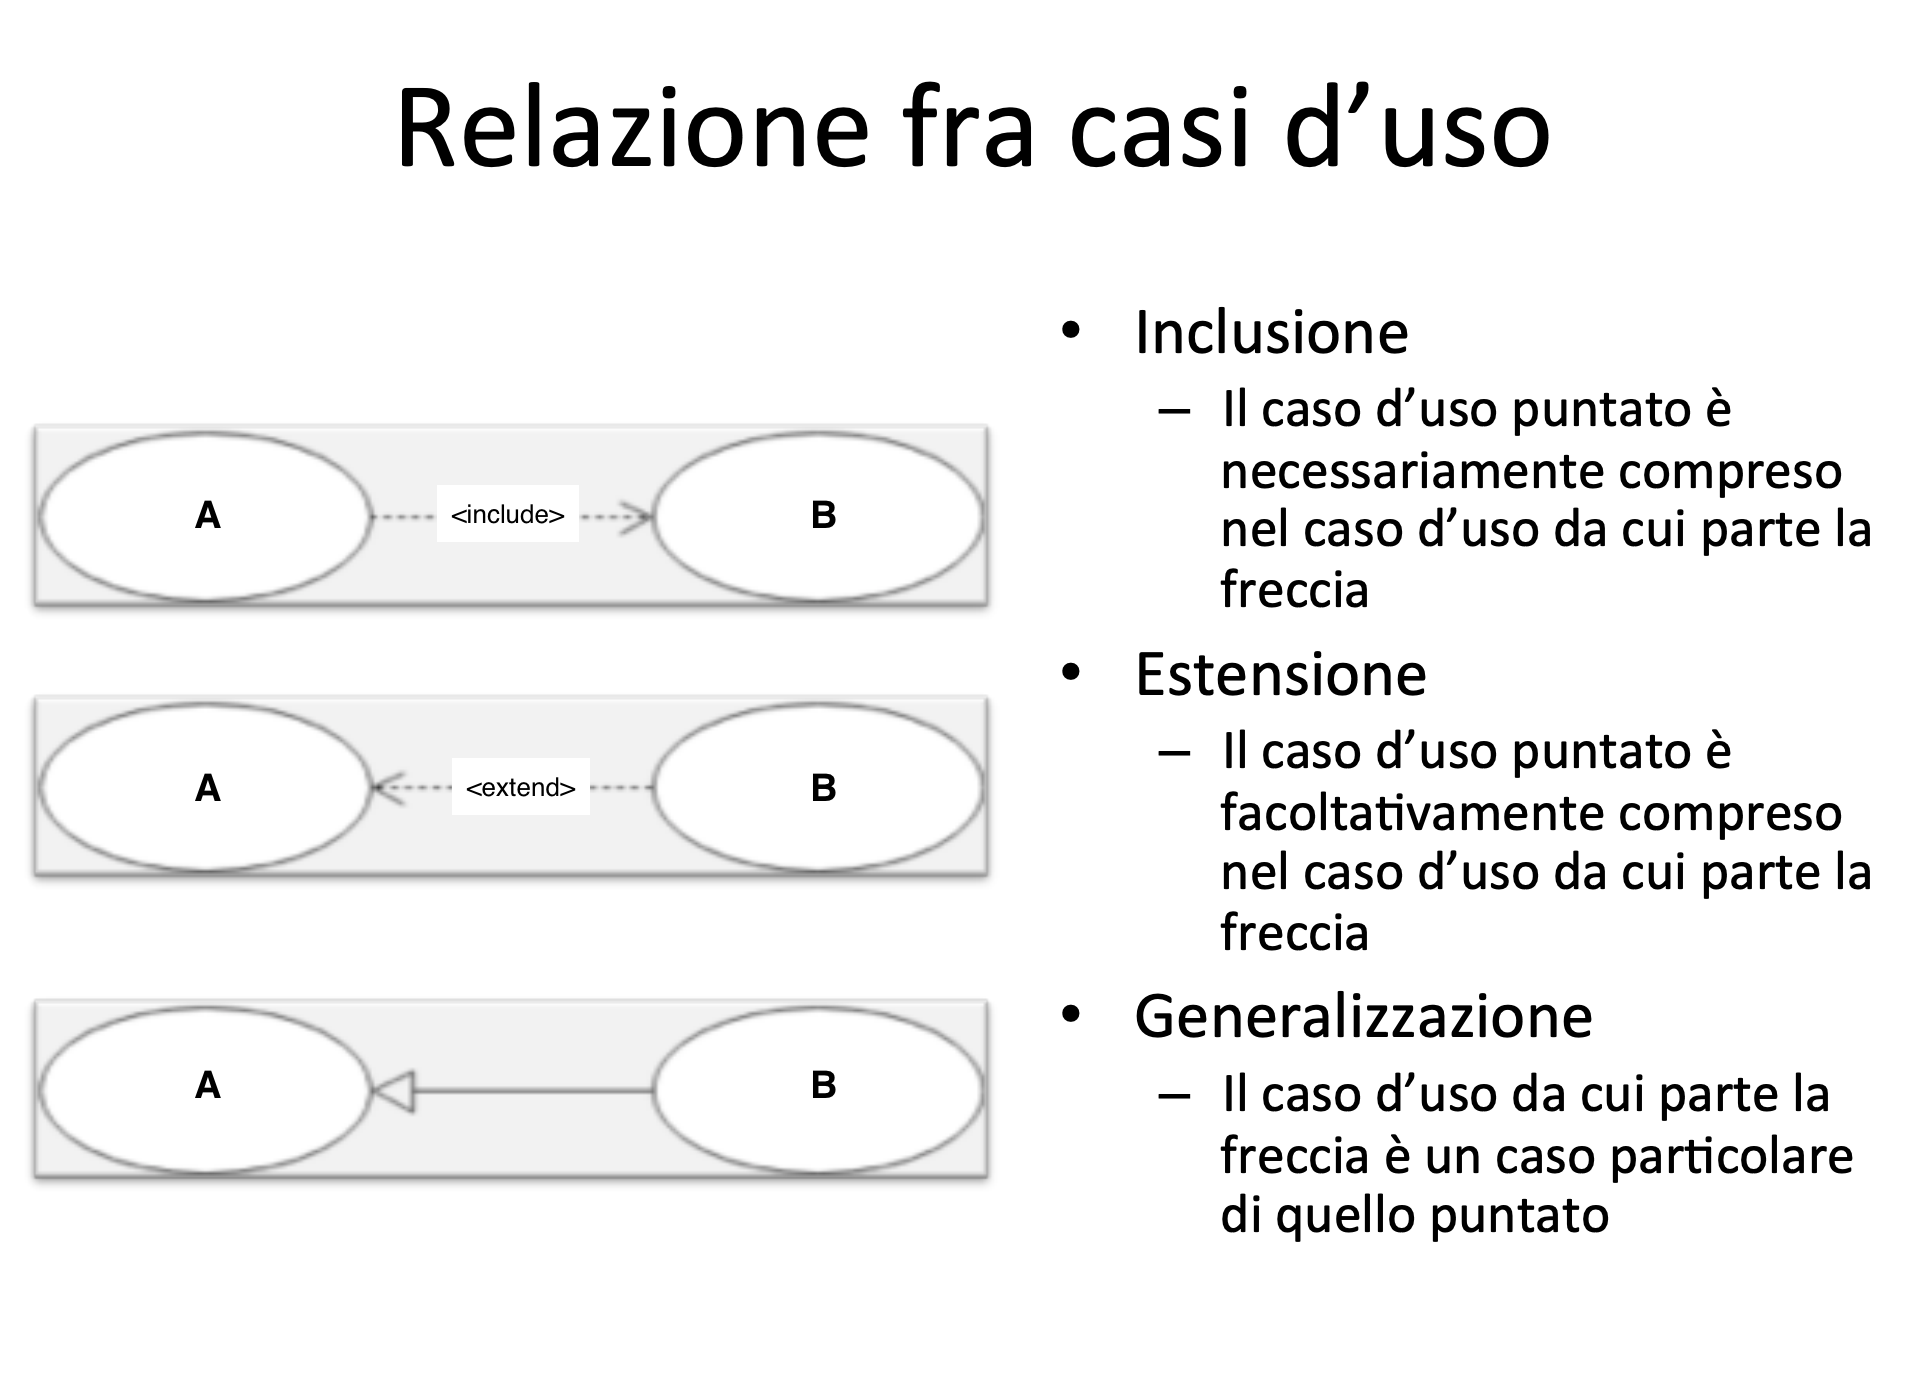
\includegraphics[width=0.8\textwidth]{immagini/uml_use_case_relazioni.png} % Immagine da Pagina 2 del tuo UML.pdf
    \caption{Rappresentazione grafica delle relazioni comuni tra Casi d'Uso in UML (Inclusione, Estensione e Generalizzazione).}
    \label{fig:uml_use_case_relazioni}
\end{figure}

\paragraph{Esempio Completo: Sistema di Ristorazione}
Un esempio pratico aiuta a consolidare la comprensione di come i casi d'uso e le loro relazioni si applichino in un contesto reale. Il diagramma seguente mostra le funzionalità di un sistema di gestione per un ristorante, illustrando le interazioni tra clienti, personale e il sistema stesso.
\begin{figure}[h!]
    \centering
    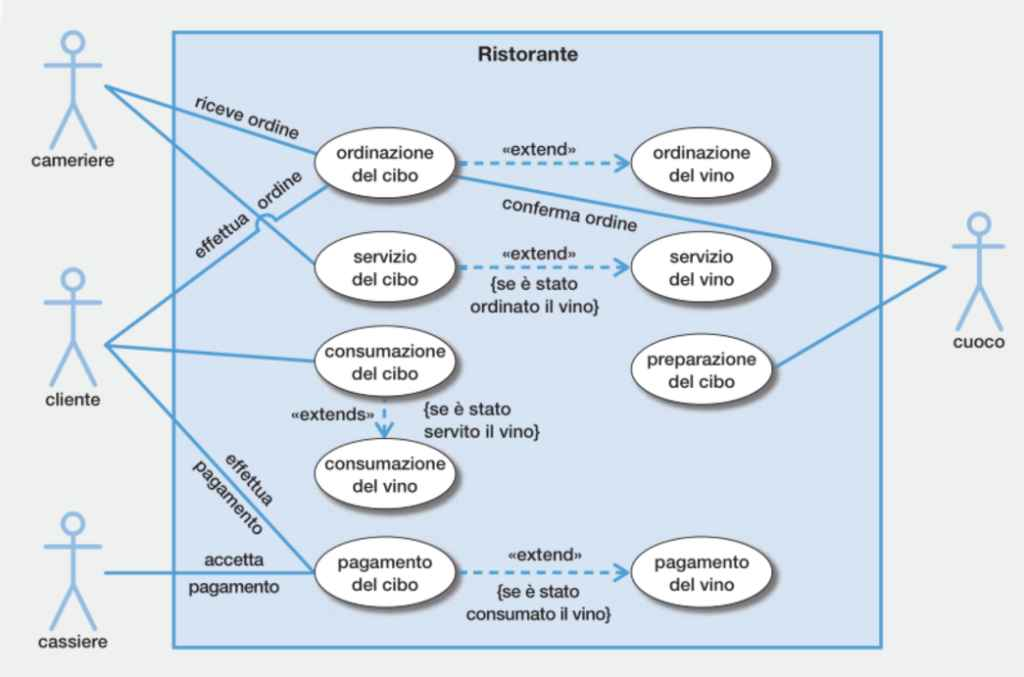
\includegraphics[width=0.9\textwidth]{immagini/diagramma_casi_uso_ristorante.jpg} % Immagine da Pagina 1 del tuo UML.pdf
    \caption{Esempio completo di Diagramma dei Casi d'Uso per un sistema di Ristorazione, che illustra le interazioni tra attori (Cameriere, Cliente, Cuoco, Cassiere) e le funzionalità del sistema.}
    \label{fig:diagramma_casi_uso_ristorante_completo}
\end{figure}

\subsubsection{Diagrammi delle Classi (Class Diagrams)}
I \textbf{Diagrammi delle Classi} sono diagrammi strutturali UML che mostrano la struttura statica di un sistema, le classi, i loro attributi (dati), i loro metodi (operazioni) e le relazioni tra le classi. Sono fondamentali per la progettazione orientata agli oggetti e per modellare il design logico del database.

\begin{itemize}
    \item \textbf{Scopo}: Modellare il design logico del sistema, la struttura del codice, le relazioni tra le classi e le dipendenze. Utile per visualizzare l'architettura del software a livello di classi.
    \item \textbf{Componenti Principali}:
    \begin{itemize}
        \item \textbf{Classe}: Rappresentata da un rettangolo diviso in tre sezioni: nome della classe, attributi (con visibilità e tipo), e metodi (con visibilità, parametri e tipo di ritorno).
        \item \textbf{Visibilità (Visibility)}: Indica l'accessibilità degli attributi e metodi, rappresentata da simboli specifici (\lstinline{+}, \lstinline{-}, \lstinline{\#}, \lstinline{\textasciitilde}).
        \item \textbf{Relazioni}: Specificano le associazioni tra le classi.
    \end{itemize}
\end{itemize}

\paragraph{Struttura Base e Attributi}
Un diagramma delle classi inizia con la rappresentazione della singola classe, evidenziando il suo nome, i suoi attributi (le proprietà) e le sue operazioni (i metodi).
\begin{figure}[h!]
    \centering
    \subcaptionbox{Struttura di una Classe (Automobile)\label{fig:class_base_automobile}}{%
        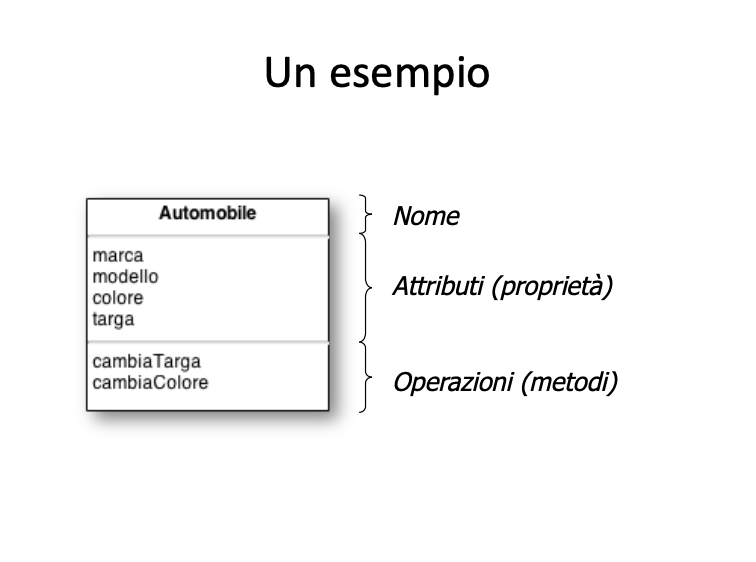
\includegraphics[width=0.45\textwidth]{immagini/uml_class_base_automobile.png}%
    }\quad
    \subcaptionbox{Classe con Metodi e Attributi (Scheda Anagrafica)\label{fig:class_scheda_anagrafica}}{%
        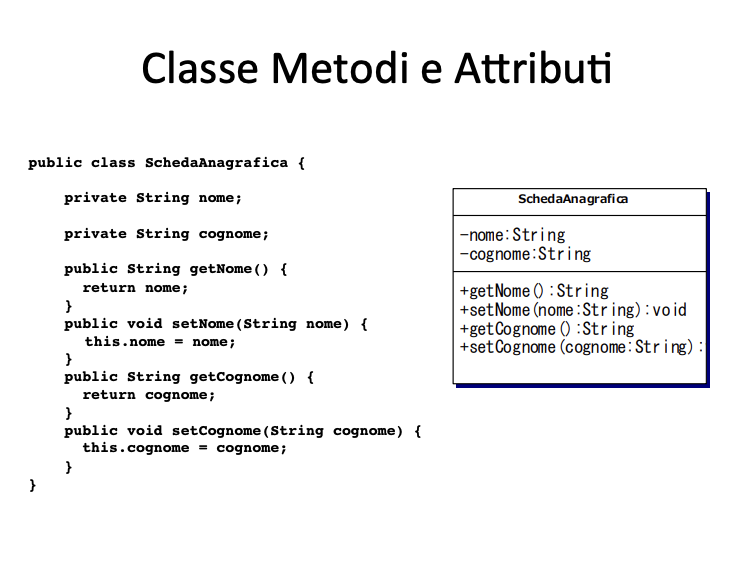
\includegraphics[width=0.45\textwidth]{immagini/uml_class_scheda_anagrafica_struttura.png}%
    }
    \caption{Esempi di rappresentazione base di una classe UML, con attributi e metodi, e come si relaziona al codice.}
    \label{fig:struttura_base_classi}
\end{figure}

L'uso di modificatori di visibilità definisce l'accessibilità di questi attributi e metodi, come mostrato nell'esempio dei Clienti e Fornitori.
\begin{figure}[h!]
    \centering
    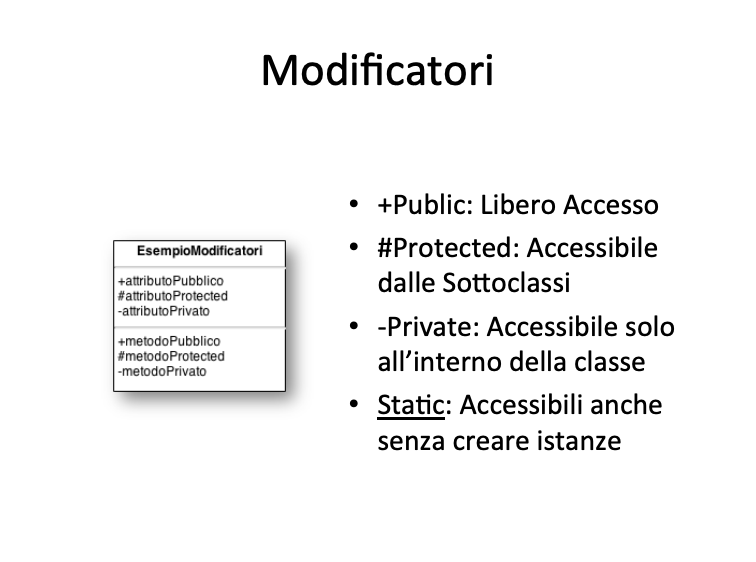
\includegraphics[width=0.7\textwidth]{immagini/uml_class_modificatori_visibilita.png}
    \caption{Esempio di Diagramma delle Classi che illustra l'uso dei modificatori di visibilità (public, private, protected) per attributi e metodi.}
    \label{fig:class_modificatori}
\end{figure}

\paragraph{Relazioni di Generalizzazione (Ereditarietà)}
La generalizzazione indica che una classe (sottoclasse) eredita proprietà e comportamenti da un'altra classe (superclasse). Questo promuove il riutilizzo del codice.
\begin{figure}[h!]
    \centering
    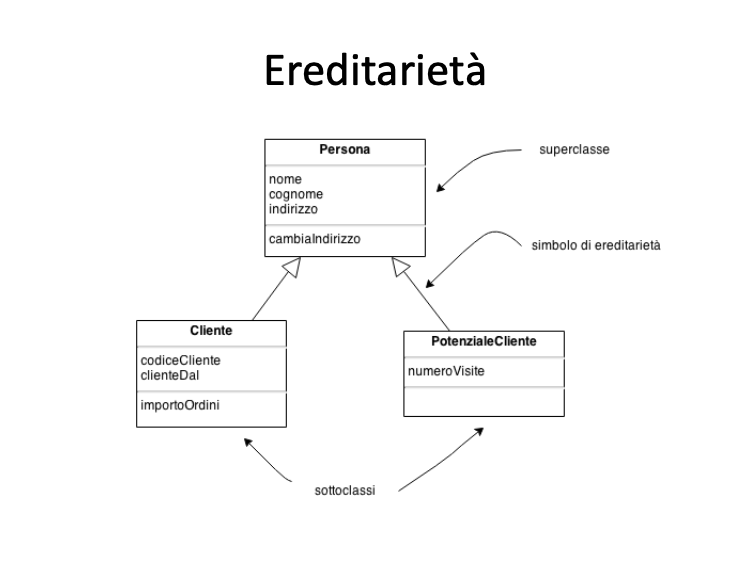
\includegraphics[width=0.7\textwidth]{immagini/uml_class_ereditarieta_generica.png}
    \caption{Esempio di Diagramma delle Classi che mostra la relazione di ereditarietà tra le classi Persona, Cliente e Potenziale Cliente.}
    \label{fig:class_ereditarieta}
\end{figure}
In contesti come Java, dove l'ereditarietà multipla non è ammessa (a differenza di C++), le interfacce vengono utilizzate per ovviare a questa limitazione, permettendo a una classe di implementare più interfacce.
\begin{figure}[h!]
    \centering
    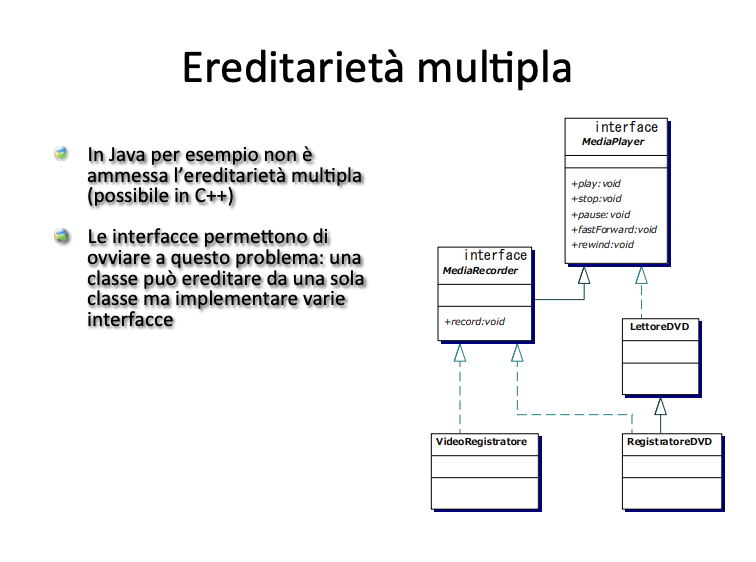
\includegraphics[width=0.7\textwidth]{immagini/uml_class_ereditarieta_multipla_interfacce.png}
    \caption{Esempio di Diagramma delle Classi che illustra come le interfacce consentono di simulare l'ereditarietà multipla in linguaggi che non la supportano nativamente.}
    \label{fig:class_ereditarieta_multipla}
\end{figure}

\paragraph{Relazioni Strutturali: Aggregazione e Composizione}
Aggregazione e composizione sono forme specifiche di associazione che esprimono relazioni "parte di" tra classi, distinguendosi per la dipendenza esistenziale della parte rispetto al tutto.
\begin{itemize}
    \item \textbf{Aggregazione}: Rappresenta una relazione uno a molti in cui l'oggetto "parte" può esistere indipendentemente dall'oggetto "tutto" (es. un libro può esistere senza una mensola specifica). Viene rappresentata con una freccia con la punta a diamante vuota all'estremità del "tutto".
    \item \textbf{Composizione}: Una forma più forte di aggregazione, che implica una esclusività. La "parte" non può esistere da sola senza il "tutto", e la distruzione del "tutto" comporta la distruzione delle "parti" (es. una pagina non può esistere senza il suo libro). Il diamante si disegna pieno.
\end{itemize}
\begin{figure}[h!]
    \centering
    \subcaptionbox{Esempio di Aggregazione (Mensola e Libro)\label{fig:class_aggregazione_esempio}}{%
        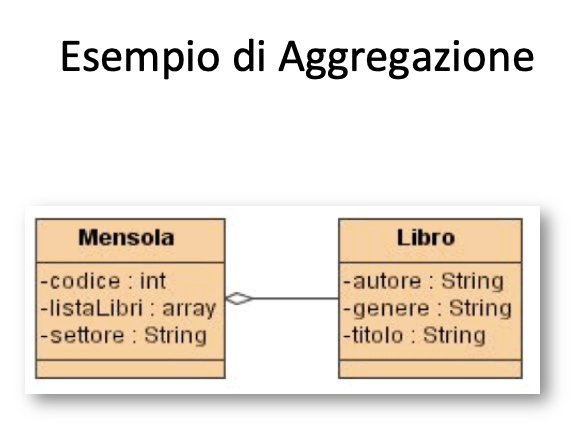
\includegraphics[width=0.45\textwidth]{immagini/uml_class_aggregazione_esempio.png}%
    }\quad
    \subcaptionbox{Esempio di Composizione (Libro e Pagina)\label{fig:class_composizione_esempio}}{%
        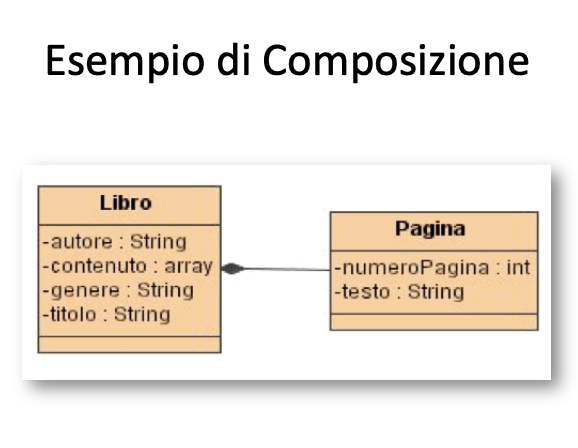
\includegraphics[width=0.45\textwidth]{immagini/uml_class_composizione_esempio.png}%
    }
    \caption{Confronto visivo tra Aggregazione e Composizione nei Diagrammi delle Classi UML.}
    \label{fig:class_aggregazione_composizione}
\end{figure}

\paragraph{Esempi Complessi di Diagrammi delle Classi}
Per illustrare l'applicazione di queste relazioni in contesti più ampi, consideriamo sistemi con diverse classi interconnesse, come un sistema e-commerce o un'applicazione di chat. Questi esempi mostrano come le classi interagiscono per formare un sistema coerente.
\begin{figure}[h!]
    \centering
    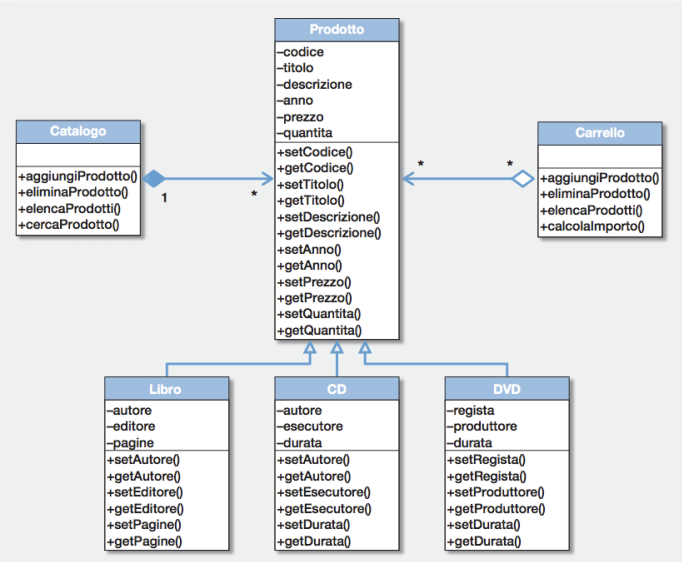
\includegraphics[width=0.9\textwidth]{immagini/uml_class_sistema_e_commerce.png} % Assicurati che l'immagine sia salvata con questo nome e percorso
    \caption{Diagramma delle Classi per un sistema di gestione prodotti/catalogo/carrello, che illustra varie classi e le loro relazioni (es. Prodotto, Carrello, DVD, Libro).}
    \label{fig:class_sistema_e_commerce}
\end{figure}
\begin{figure}[h!]
    \centering
    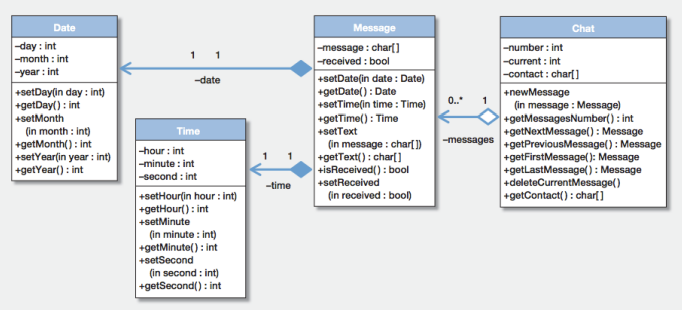
\includegraphics[width=0.9\textwidth]{immagini/uml_class_sistema_chat_corretto.png} % Assicurati che l'immagine sia salvata con questo nome e percorso
    \caption{Diagramma delle Classi per un sistema di Chat, che mostra le interazioni tra classi come Utente, Chat e Messaggio, e le loro molteplicità.}
    \label{fig:class_sistema_chat}
\end{figure}

\subsubsection{Diagrammi di Sequenza (Sequence Diagrams)}
Un \textbf{Diagramma di Sequenza}, o in inglese \textit{Sequence Diagram}, è un diagramma appartenente alla famiglia del linguaggio \textbf{UML (Unified Modeling Language)}, che viene utilizzato principalmente per rappresentare le interazioni tra gli oggetti, rispettando l'ordine sequenziale in cui avvengono questi scambi di messaggi. Sono utili non solo agli sviluppatori per modellare il comportamento di un'applicazione, ma anche ai dirigenti di un'azienda, in quanto possono riprodurre il comportamento dei vari elementi del sistema che costituiscono il business, mostrando come interagiscono tra loro. Lo staff tecnico di un'organizzazione potrebbe avvalersi di questi diagrammi per documentare un comportamento. Ad esempio, durante la fase di progettazione, architetti e sviluppatori possono utilizzare questo schema per aggiungere o eliminare le interazioni tra le componenti del sistema.

È possibile utilizzare i diagrammi di sequenza a diversi livelli durante il processo di sviluppo:
\begin{itemize}
    \item Nella fase di \textbf{analisi}, possono aiutare ad identificare le classi di cui un sistema ha bisogno e ciò che gli oggetti di classe fanno nelle interazioni.
    \item Nella fase di \textbf{progettazione}, spiegano come il sistema funziona per compiere le interazioni.
    \item Durante la costruzione di un'\textbf{architettura di un sistema}, è possibile utilizzarli per mostrare il funzionamento dei modelli di progettazione ed i meccanismi che il sistema utilizza.
\end{itemize}
Uno dei principali usi del diagramma è quello di raffinare, in uno o più diagrammi, i requisiti espressi nei diagrammi dei casi d'uso UML, che vengono usati per la descrizione delle funzioni o servizi offerti da un sistema, così come sono percepiti e utilizzati dagli attori che interagiscono col sistema stesso.
Lo scopo principale è quello di definire sequenze di eventi che portano a qualche risultato desiderato. L'attenzione si concentra sull'ordine in cui si verificano i messaggi piuttosto che sul loro contenuto. Il diagramma trasmette queste informazioni lungo le dimensioni orizzontali e verticali:
\begin{itemize}
    \item In \textbf{verticale}, dall'alto verso il basso, è evidenziata la sequenza temporale dei messaggi secondo l'ordine in cui si verificano.
    \item In \textbf{orizzontale}, da sinistra a destra, le istanze degli oggetti a cui sono inviati i messaggi.
\end{itemize}

\paragraph{Componenti Principali dei Diagrammi di Sequenza}
\begin{itemize}
    \item \textbf{Lifeline (Linea di Vita)}: Rappresenta la partecipazione di un oggetto o attore all'interazione, mostrata come una linea verticale tratteggiata. In cima alla lifeline c'è un rettangolo (per gli oggetti) o un omino (per gli attori).
    \item \textbf{Attore}: Utente o sistema esterno che avvia o partecipa all'interazione.
    \item \textbf{Messaggio}: Una comunicazione o chiamata di metodo tra lifeline, rappresentata da una freccia orizzontale. Possono essere:
    \begin{itemize}
        \item \textbf{Sincroni}: Freccia piena, indica una chiamata bloccante in attesa di risposta.
        \item \textbf{Asincroni}: Freccia con punta aperta, indica una chiamata non bloccante.
        \item \textbf{Risposta}: Freccia tratteggiata, indica il ritorno di un valore o la fine di una chiamata sincrona.
    \end{itemize}
    \item \textbf{Barra di Attivazione (Activation Bar/Execution Occurrence)}: Un rettangolo sottile posizionato verticalmente sulla lifeline, che indica il periodo di tempo durante il quale un oggetto è attivo e sta eseguendo un'operazione o aspettando una risposta.
    \item \textbf{Frammenti Combinati (Combined Fragments)}: Costrutti per mostrare strutture di controllo logico:
    \begin{itemize}
        \item \textbf{alt (alternative)}: Per mostrare blocchi if-else.
        \item \textbf{opt (optional)}: Per mostrare un blocco if.
        \item \textbf{loop (loop)}: Per mostrare iterazioni.
        \textbf{par (parallel)}: Per mostrare esecuzioni parallele.
    \end{itemize}
\end{itemize}

\paragraph{Esempio 1: Flusso di Aggiornamento Dati in MVC}
Questo esempio illustra un tipico flusso di aggiornamento dei dati in un'architettura Model-View-Controller (MVC), mostrando le interazioni tra l'utente, la View, il Controller e il Model. È un esempio comune per descrivere come le modifiche da parte dell'utente si propagano attraverso i livelli di un'applicazione.
\begin{figure}[h!]
    \centering
    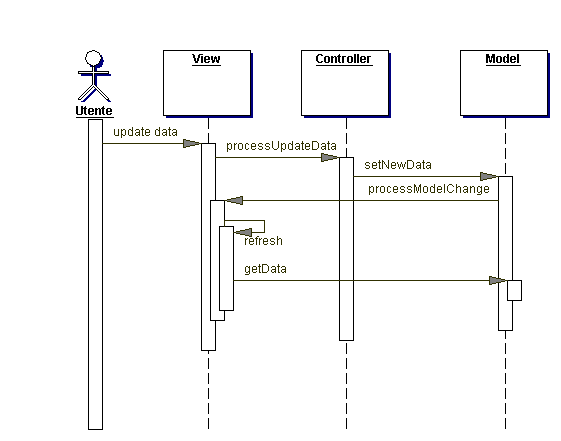
\includegraphics[width=0.8\textwidth]{immagini/uml_sequence_mvc_update.png} % Ho corretto a .png. Se la tua è .gif, cambia qui.
    \caption{Diagramma di Sequenza UML che illustra il flusso di aggiornamento dei dati in un'architettura Model-View-Controller (MVC).}
    \label{fig:diagramma_sequenza_mvc_update}
\end{figure}

\paragraph{Esempio 2: Flusso di Prestito in un Sistema Biblioteca}
Questo diagramma mostra un processo più orientato al dominio di business, come la gestione del prestito di un libro in un sistema di biblioteca. Evidenzia l'interazione tra l'utente, un gestore dei prestiti, l'entità libro, e i registri dei prestiti totali, illustrando come i sistemi gestiscono gli stati e le verifiche per completare un'operazione.
\begin{figure}[h!]
    \centering
    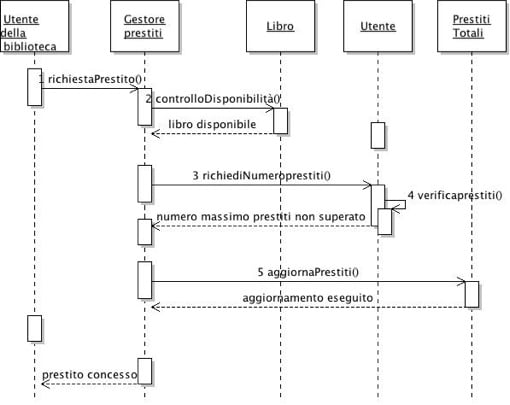
\includegraphics[width=0.8\textwidth]{immagini/uml_sequence_prestito_biblioteca.jpg} % Assicurati che il nome del file sia corretto
    \caption{Diagramma di Sequenza UML che illustra il flusso di prestito di un libro in un sistema di gestione bibliotecaria.}
    \label{fig:diagramma_sequenza_prestito_biblioteca}
\end{figure}
